\documentclass[border=5pt]{standalone}
\usepackage[T1]{fontenc}
\usepackage{helvet,courier}
\usepackage{amsmath,amssymb}
\usepackage{tikz}
\usetikzlibrary{positioning,arrows.meta,calc,backgrounds}
\renewcommand{\familydefault}{\sfdefault}

\definecolor{bgPrimary}{HTML}{E8EEF7}
\definecolor{bgInput}{HTML}{F0F4F8}
\definecolor{borderPrimary}{HTML}{6C8EBF}
\definecolor{borderAccent}{HTML}{3A6EA5}
\definecolor{arrowColor}{HTML}{4A6A8A}
\definecolor{textMain}{HTML}{243647}
\definecolor{textLight}{HTML}{526779}
\definecolor{bgProbe}{HTML}{E6F1EF}
\definecolor{probeAccent}{HTML}{548E87}

\tikzset{
  card/.style={draw=borderPrimary,fill=bgPrimary,rounded corners=3pt,
    line width=.6pt,inner sep=6pt,text=textMain,align=center,
    font=\sffamily\fontsize{8.5}{10.5}\selectfont},
  input/.style={card,fill=bgInput,text width=2.7cm,minimum height=.9cm},
  evidence/.style={card,text width=3.25cm,minimum height=2.35cm},
  merge/.style={card,draw=borderAccent,line width=.9pt,text width=3.25cm},
  metric/.style={card,fill=white,minimum width=5.9cm,minimum height=1.65cm},
  flow/.style={-{Stealth[length=4.4pt,width=3.4pt]},draw=arrowColor,
    line width=.75pt,rounded corners=3pt},
  wire/.style={draw=arrowColor,line width=.75pt,rounded corners=3pt},
  heading/.style={anchor=west,font=\sffamily\bfseries\fontsize{10}{12}\selectfont,text=textMain},
  note/.style={font=\sffamily\fontsize{8}{10}\selectfont,text=textLight,align=center},
  title/.style={font=\sffamily\bfseries\fontsize{9.3}{11}\selectfont,text=textMain,anchor=west},
  detail/.style={font=\sffamily\fontsize{8.5}{10.5}\selectfont,text=textLight,anchor=west,align=left},
  score/.style={font=\sffamily\bfseries\fontsize{10}{12}\selectfont,text=borderAccent,anchor=east}
}
\begin{document}
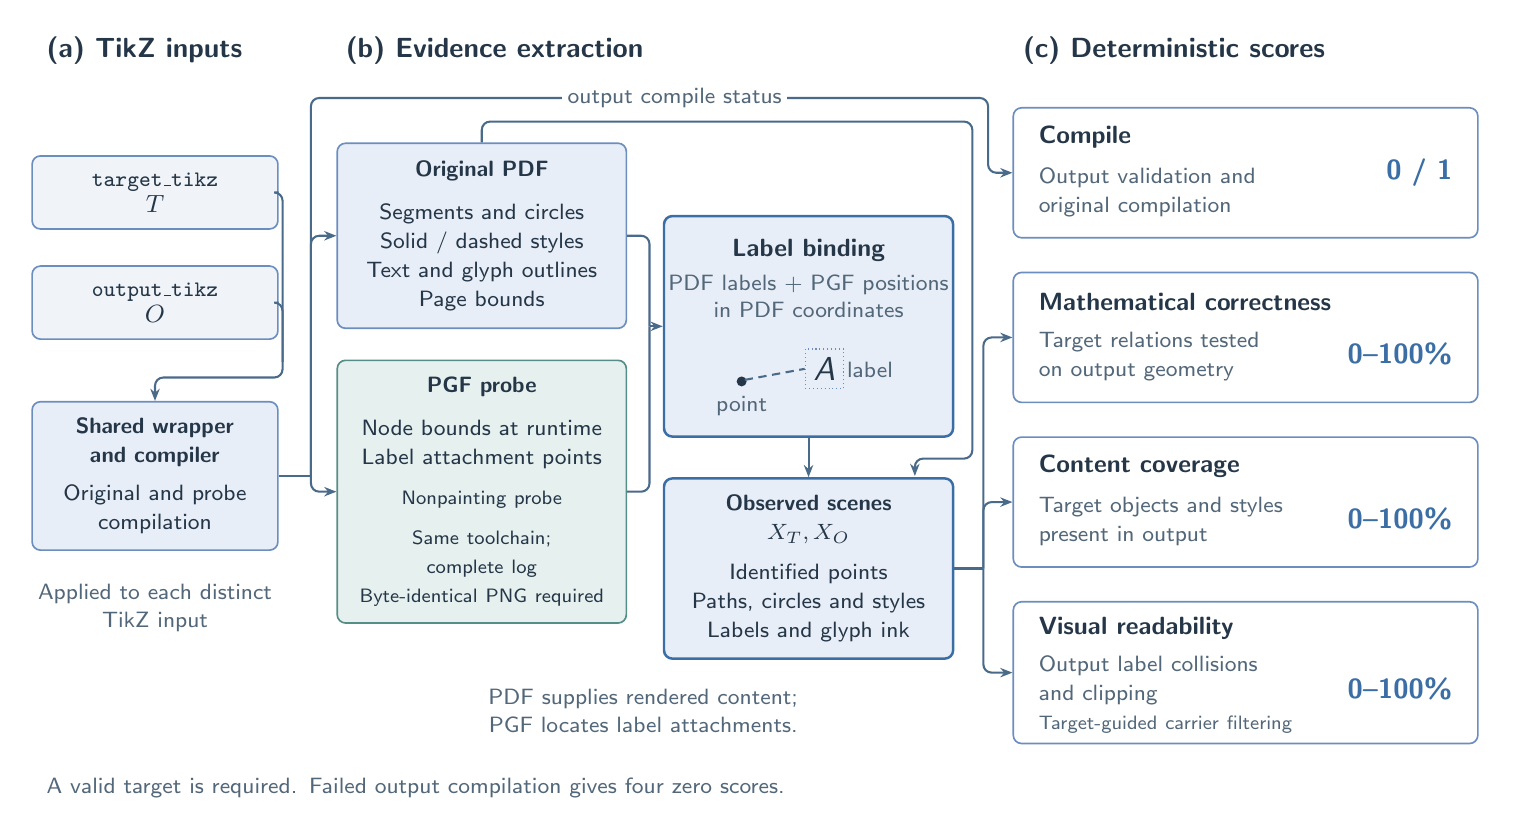
\begin{tikzpicture}
\node[heading] at (0,10.5) {(a) TikZ inputs};
\node[heading] at (3.8,10.5) {(b) Evidence extraction};
\node[heading] at (12.4,10.5) {(c) Deterministic scores};

\node[input] (target) at (1.5,8.7) {\texttt{target\_tikz}\\[-1pt]{\small $T$}};
\node[input,below=.45cm of target] (output) {\texttt{output\_tikz}\\[-1pt]{\small $O$}};
\node[card,text width=2.7cm,minimum height=1.5cm] (compiler) at (1.5,5.1)
  {\textbf{Shared wrapper}\\\textbf{and compiler}\\[4pt]
   {\footnotesize Original and probe\\compilation}};
\coordinate (inputjoin) at (3.12,6.55);
\draw[wire] (target.east) -- (3.12,8.7) -- (inputjoin);
\draw[wire] (output.east) -- (inputjoin |- output.east) -- (inputjoin);
\draw[flow] (inputjoin) -- (3.12,6.35) -| (compiler.north);
\node[note,text width=3cm,below=.3cm of compiler] {Applied to each distinct\\TikZ input};

\node[evidence] (pdf) at (5.65,8.15) {
  \textbf{Original PDF}\\[5pt]
  Segments and circles\\
  Solid / dashed styles\\
  Text and glyph outlines\\
  Page bounds
};
\node[evidence,fill=bgProbe,draw=probeAccent,minimum height=3.0cm] (probe) at (5.65,4.9) {
  \textbf{PGF probe}\\[5pt]
  Node bounds at runtime\\
  Label attachment points\\[4pt]
  {\fontsize{7.5}{9}\selectfont Nonpainting probe}\\[4pt]
  {\fontsize{7.5}{9}\selectfont Same toolchain; complete log}\\
  {\fontsize{7.5}{9}\selectfont Byte-identical PNG required}
};
\coordinate (compilex) at (3.48,0);
\coordinate (compilefork) at (compilex |- compiler.east);
\draw[wire] (compiler.east) -- (compilefork);
\draw[flow] (compilefork) |- (pdf.west);
\draw[flow] (compilefork) |- (probe.west);

\node[merge,minimum height=2.8cm] (binding) at (9.8,7.0) {};
\node[title,anchor=center] at (9.8,7.96) {Label binding};
\node[note] at (9.8,7.38) {PDF labels + PGF positions\\in PDF coordinates};
% The visible glyph is offset from the mathematical point.
\fill[textMain] (8.95,6.3) circle[radius=1.8pt];
\node[note] at (8.95,5.99) {point};
\node[draw=borderPrimary,densely dotted,inner sep=3pt,
  font=\sffamily\itshape\fontsize{12}{12}\selectfont,text=textMain] (glyph) at (10.0,6.46) {A};
\draw[wire,densely dashed] (8.99,6.32) -- (glyph.west);
\node[note] at (10.58,6.45) {label};

\coordinate (evidencejoin) at (7.78,7.0);
\draw[wire] (pdf.east) -- (7.78,8.15) -- (evidencejoin);
\draw[wire] (probe.east) -- (7.78,4.9) -- (evidencejoin);
\draw[flow] (evidencejoin) -- (binding.west);

\node[merge,minimum height=2.2cm,below=.5cm of binding] (scene) {
  \textbf{Observed scenes}\\$X_T,X_O$\\[4pt]
  Identified points\\
  Paths, circles and styles\\
  Labels and glyph ink
};
\draw[flow] (binding.south) -- (scene.north);
% Rendered paths and glyph ink bypass point-label binding.
\draw[flow] (pdf.north) -- (5.65,9.6) -- (11.88,9.6)
  -- (11.88,5.32) -- (11.15,5.32) -- (11.15,5.1);
\node[note,text width=7.5cm] at (7.7,2.12)
  {PDF supplies rendered content; PGF locates label attachments.};

\node[metric] (compile) at (15.35,8.95) {};
\node[title] at ([xshift=6pt,yshift=13pt]compile.west) {Compile};
\node[detail,text width=4.5cm] at ([xshift=6pt,yshift=-7pt]compile.west)
  {Output validation and\\original compilation};
\node[score] at ([xshift=-6pt]compile.east) {0 / 1};

\node[metric,below=.42cm of compile] (math) {};
\node[title] at ([xshift=6pt,yshift=13pt]math.west) {Mathematical correctness};
\node[detail,text width=4.4cm] at ([xshift=6pt,yshift=-7pt]math.west)
  {Target relations tested\\on output geometry};
\node[score] at ([xshift=-6pt,yshift=-6pt]math.east) {0--100\%};

\node[metric,below=.42cm of math] (coverage) {};
\node[title] at ([xshift=6pt,yshift=13pt]coverage.west) {Content coverage};
\node[detail,text width=4.35cm] at ([xshift=6pt,yshift=-7pt]coverage.west)
  {Target objects and styles\\present in output};
\node[score] at ([xshift=-6pt,yshift=-6pt]coverage.east) {0--100\%};

\node[metric,minimum height=1.8cm,below=.42cm of coverage] (readability) {};
\node[title] at ([xshift=6pt,yshift=16pt]readability.west) {Visual readability};
\node[detail,text width=4.25cm] at ([xshift=6pt,yshift=-8pt]readability.west)
  {Output label collisions\\and clipping\\
   {\fontsize{7.2}{9}\selectfont Target-guided carrier filtering}};
\node[score] at ([xshift=-6pt,yshift=-6pt]readability.east) {0--100\%};

% Compilation bypasses the geometric evidence and comparison stages.
\draw[flow] (compilefork) -- (3.48,9.9) -- (12.08,9.9) |- (compile.west);
\node[note,fill=white,inner sep=2pt] at (8.1,9.9) {output compile status};

% Both observed scenes are available to the three downstream checks.
\coordinate (forkx) at (12.02,0);
\coordinate (scenefork) at (forkx |- scene.east);
\draw[wire] (scene.east) -- (scenefork);
\draw[flow] (scenefork) |- (math.west);
\draw[flow] (scenefork) |- (coverage.west);
\draw[flow] (scenefork) |- (readability.west);

\node[note,anchor=north west,text width=18.2cm,align=left] at (0,1.38) {
  A valid target is required. Failed output compilation gives four zero scores.
};
\end{tikzpicture}
\end{document}
